%% abtex2-modelo-artigoresu, v-1.9.6 laurocesar
%% Copyright 2012-2016 by abnTeX2 group at http://www.abntex.net.br/ 
%%
%% This work may be distributed and/or modified under the
%% conditions of the LaTeX Project Public License, either version 1.3
%% of this license or (at your option) any later version.
%% The latest version of this license is in
%%   http://www.latex-project.org/lppl.txt
%% and version 1.3 or later is part of all distributions of LaTeX
%% version 2005/12/01 or later.
%%
%% This work has the LPPL maintenance status `maintained'.
%% 
%% The Current Maintainer of this work is the abnTeX2 team, led
%% by Lauro César Araujo. Further information are available on 
%% http://www.abntex.net.br/
%%
%% This work consists of the files abntex2-modelo-artigo.tex and
%% abntex2-modelo-references.bib
%%

% ------------------------------------------------------------------------
% ------------------------------------------------------------------------
% abnTeX2: Modelo de Artigo Acadêmico em conformidade com
% ABNT NBR 6022:2003: Informação e documentação - Artigo em publicação 
% periódica científica impressa - Apresentação
% ------------------------------------------------------------------------
% ------------------------------------------------------------------------

\documentclass[
	% -- opções da classe memoir --
	article,			% indica que é um artigo acadêmico
	11pt,				% tamanho da fonte
	oneside,			% para impressão apenas no recto. Oposto a twoside
	a4paper,			% tamanho do papel. 
	% -- opções da classe abntex2 --
	%chapter=TITLE,		% títulos de capítulos convertidos em letras maiúsculas
	%section=TITLE,		% títulos de seções convertidos em letras maiúsculas
	%subsection=TITLE,	% títulos de subseções convertidos em letras maiúsculas
	%subsubsection=TITLE % títulos de subsubseções convertidos em letras maiúsculas
	% -- opções do pacote babel --
	english,			% idioma adicional para hifenização
	brazil,				% o último idioma é o principal do documento
	sumario=tradicional
	]{abntex2}


% ---
% PACOTES
% ---

% ---
% Pacotes fundamentais 
% ---
\usepackage{lmodern}			% Usa a fonte Latin Modern
\usepackage[T1]{fontenc}		% Selecao de codigos de fonte.
\usepackage[utf8]{inputenc}		% Codificacao do documento (conversão automática dos acentos)
\usepackage{indentfirst}		% Indenta o primeiro parágrafo de cada seção.
\usepackage{nomencl} 			% Lista de simbolos
\usepackage{color}				% Controle das cores
\usepackage{graphicx}			% Inclusão de gráficos
\usepackage{microtype} 			% para melhorias de justificação
% ---
\usepackage[brazil]{babel}
\usepackage{listings}
\usepackage{color}		
% ---
% Pacotes adicionais, usados apenas no âmbito do Modelo Canônico do abnteX2
% ---
\usepackage{lipsum}				% para geração de dummy text
% ---
		
% ---
% Pacotes de citações
% ---
\usepackage[brazilian,hyperpageref]{backref}	 % Paginas com as citações na bibl
\usepackage[alf]{abntex2cite}	% Citações padrão ABNT
% ---

% ---
% Configurações do pacote backref
% Usado sem a opção hyperpageref de backref
\renewcommand{\backrefpagesname}{Citado na(s) página(s):~}
% Texto padrão antes do número das páginas
\renewcommand{\backref}{}
% Define os textos da citação
%\renewcommand*{\backrefalt}[4]{
%	\ifcase #1 %
%		Nenhuma citação no texto.%
%	\or
%		Citado na página #2.%
%	\else
%		Citado #1 vezes nas páginas #2.%
%	\fi}%
% ---

% ---
% Informações de dados para CAPA e FOLHA DE ROSTO
% ---
\titulo{Wiring, Arduíno e o ARM. Como estas tecnologias estão relacionadas}
\autor{Ricardo Aparecido Bezerra Elias da Silva - 15203158}
\local{Brasil}
\data{2018}
% ---

% ---
% Configurações de aparência do PDF final

% alterando o aspecto da cor azul
\definecolor{blue}{RGB}{41,5,195}

% informações do PDF
\makeatletter
\hypersetup{
     	%pagebackref=true,
		pdftitle={\@title}, 
		pdfauthor={\@author},
    	pdfsubject={Modelo de artigo científico com abnTeX2},
	    pdfcreator={LaTeX with abnTeX2},
		pdfkeywords={abnt}{latex}{abntex}{abntex2}{atigo científico}, 
		colorlinks=true,       		% false: boxed links; true: colored links
    	linkcolor=blue,          	% color of internal links
    	citecolor=blue,        		% color of links to bibliography
    	filecolor=magenta,      		% color of file links
		urlcolor=blue,
		bookmarksdepth=4
}
\makeatother
% --- 

% ---
% compila o indice
% ---
\makeindex
% ---

% ---
% Altera as margens padrões
% ---
\setlrmarginsandblock{3cm}{3cm}{*}
\setulmarginsandblock{3cm}{3cm}{*}
\checkandfixthelayout
% ---

% --- 
% Espaçamentos entre linhas e parágrafos 
% --- 

% O tamanho do parágrafo é dado por:
\setlength{\parindent}{1.3cm}

% Controle do espaçamento entre um parágrafo e outro:
\setlength{\parskip}{0.2cm}  % tente também \onelineskip

% Espaçamento simples
\SingleSpacing

% ----
% Início do documento
% ----
\begin{document}

% Seleciona o idioma do documento (conforme pacotes do babel)
%\selectlanguage{english}
\selectlanguage{brazil}

% Retira espaço extra obsoleto entre as frases.
\frenchspacing 

% ----------------------------------------------------------
% ELEMENTOS PRÉ-TEXTUAIS
% ----------------------------------------------------------

%---
%
% Se desejar escrever o artigo em duas colunas, descomente a linha abaixo
% e a linha com o texto ``FIM DE ARTIGO EM DUAS COLUNAS''.
%\twocolumn[    		% INICIO DE ARTIGO EM DUAS COLUNAS
%
%---
% página de titulo
\maketitle

% resumo em português
\begin{resumoumacoluna}
 

Lorem ipsum dolor sit amet, consectetur adipiscing elit. Donec diam elit, pellentesque sit amet nunc at, eleifend elementum eros. Praesent pulvinar nibh turpis, eget faucibus lectus efficitur vel. Vivamus ut nisi risus. Class aptent taciti sociosqu ad litora torquent per conubia nostra, per inceptos himenaeos. Proin sed quam vitae risus vulputate auctor eget ut odio. Praesent eleifend porttitor purus, in ullamcorper neque placerat quis. Praesent fringilla enim lectus, vitae varius nunc cursus vitae. Praesent vitae ex vitae massa aliquet fringilla. Interdum et malesuada fames ac ante ipsum primis in faucibus. Nulla vehicula mi risus, eu sollicitudin dui bibendum non. Nam nec orci nec enim dapibus ullamcorper nec sed sapien.

Sed tincidunt, nunc vulputate lobortis commodo, sem massa auctor quam, et egestas erat dui in dui. Aenean efficitur, urna vitae condimentum placerat, dui dolor lobortis dui, nec molestie velit purus sed lorem. Quisque eu nunc tellus. Integer in risus accumsan, vehicula arcu quis, interdum velit. Aenean molestie congue dolor, at suscipit odio iaculis quis. Vestibulum posuere, leo vel aliquet pellentesque, risus metus rhoncus metus, at lobortis diam ipsum vel neque. Vivamus augue arcu, facilisis eu facilisis fermentum, eleifend non urna. Integer faucibus, odio eget dictum rhoncus, nisi augue volutpat libero, vitae cursus justo ex et metus. Ut eleifend lectus ut quam rhoncus blandit. Nunc maximus elit velit, varius facilisis ligula rutrum quis. Integer nec interdum purus. Duis finibus urna a elementum fringilla. Quisque eget porta mi, nec fringilla tellus. Quisque lacinia leo at diam tincidunt ornare. Suspendisse potenti. Nulla facilisi. Mauris. 
 
 \vspace{\onelineskip}
 
 \noindent
 \textbf{Palavras-chave}: Wiring, Processing, Arduíno.
\end{resumoumacoluna}

%]  			% FIM DE ARTIGO EM DUAS COLUNAS
% ---

% ----------------------------------------------------------
% ELEMENTOS TEXTUAIS
% ----------------------------------------------------------
\textual

% ----------------------------------------------------------
% Introdução
% ----------------------------------------------------------
\section[Wiring]{Wiring}

\subsection{Início do Wiring}
Barragán, um dos criadores do Wiring, define sua criação como "um ambiente de programação e uma placa de entrada / saída de prototipagem eletrônica para explorar as artes eletrônicas e a mídia tangível"\cite{Barragan2004}.

O projeto Wiring foi iniciado em 2003 durante o mestrado de Barragán pela Interaction Design Institute Ivrea (IDII), Italia \footnote{\url{http://wiki.wiring.co/wiki/About}}. Sua idéia era disponibilizar a designers e artistas uma plataforma eletrônica de fácil utilização, retirando a necessidade de estudo afundo em linguagens de programação e eletrônica fazendo o usuário ter maior foco no que de fato é sua expertise. Esta facilidade também poderia ser aplicada no ensino de programação e prototipagem nas escolas.

Barragán se formou com distinção, o único a conseguir tal fação na IDII em 2004.

No outono do mesmo ano, o Wiring foi utilizado em curso de inverno de computação física na IDII, sendo o nome do projeto Stranger Familiar, ministrado por nomes como Massimo Banzi, Heather Martin, Yaniv Steiner, Reto Wettach. Neste projeto foi proposto a criação de objetos domésticos incomuns porém interessantíssimos\footnote{\url{http://wiring.org.co/exhibition/images/book01.pdf}}

\subsection{Wiring e o Processing}

O Processing foi criado em 2001 por Ben Fry e Casey Reas. Seu objetivo era tornar a programação mais visual, facilitando a entrada de não-programadores ao meio da computação, principalmente voltado a artes e design.\cite{reas2007processing} A linguagem tem por base as capacidades gráficas da linguagem de programação Java. O Wiring foi desenvolvido através do Processing.

"Processing, como um subconjunto na linguagem Java, traz aos usuários uma interface de aplicativo independente da tecnologia na qual ele é usado, mantendo um nível de abstração que permite aos usuários aprender os fundamentos da programação de computadores e se concentrar em seus projetos ao invés de questões ou especificidades tecnológicas de uma plataforma. A linguagem de programação Java oferece uma sintaxe muito semelhante a C, C ++, Javascript ou Flash Actionscript, possibilitando a construção de programas e algoritmos que podem ser facilmente traduzidos para diferentes linguagens e ambientes. Isso faz do Processing uma ferramenta muito interessante para ensinar e aprender programação de computadores."\cite{Barragan2004}.

\subsection{Wiring e o Arduíno}

Ao contrário da relação entre Wiring e Processing, há uma grande discussão sobre o reconhecimento de o Arduíno ser uma derivação do Wiring.
Na página de créditos do Arduíno \footnote{\url{http://wiki.wiring.co/wiki/About}}, os autores informam que o Arduíno "(...)deriva do Wiring, uma plataforma construída por Hernando Barragán como sua tese de mestrado na Interaction-Ivrea" mas reforçam que o Wiring e, por sua vez, o Arduíno são derivados de um projeto chamado Massimo's Programma2003 (Figura \ref{programma2003}) e Processing, o último reconhecido por Barragán. 

\begin{figure}[htb]
	\caption{\label{programma2003}Placa Programma2003 projetada por Massimo Banzi em 2003}
	\begin{center}
	    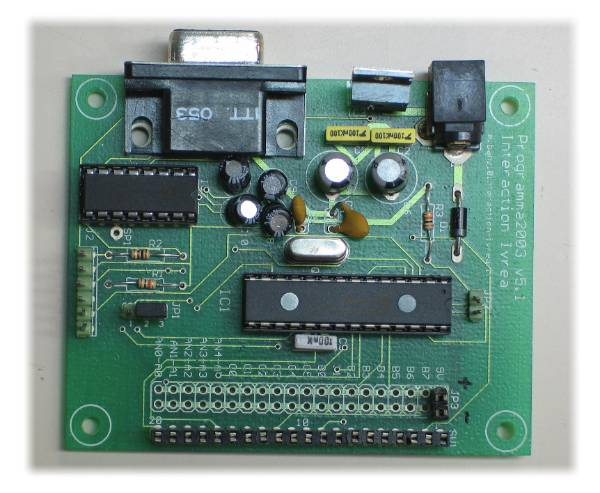
\includegraphics[scale=0.3]{refs/Programma2003}
	\end{center}
	%\legend{Fonte: Site da 3GPP}
\end{figure}

Já o criador do Wiring, criou uma página de nome "The Untold History of Arduino" \footnote{\url{https://arduinohistory.github.io/}} onde explica, em tom de crítica, diversos tópicos sobre o Arduíno.

%https://arduinohistory.github.io/
%http://wiki.wiring.co/wiki/About
%http://wiring.org.co/exhibition/images/book01.pdf
%https://www.arduino.cc/en/Main/Credits
\section[O Hardware]{O Hardware}

O hardware Wiring (\autoref{wiringS}) é uma pequena placa de circuito com um microcontrolador atmega644p, construída com base na linguagem Processing. Abaixo algumas características básicas desta placa: 

\begin{alineas}
    \item Pinos digitais de entrada e saída
    \item Pino analógico de entrada
    \item Pino PWM\footnote{\url{https://www.citisystems.com.br/pwm/}} de saída
    \item Porta serial (disponível através do conector USB)
    \item Fonte de alimentação de 7 a 12 Volts
\end{alineas}

Possui aplicações em ensino de eletrônica, ensino de programação de computadores, mídia tangível, arte interativa, etc.

Para mais características consultar o site do fabricante\footnote{\url{http://wiring.org.co/hardware/}}

\begin{figure}[htb]
	\caption{\label{wiringS}Placa Wiring S}
	\begin{center}
	    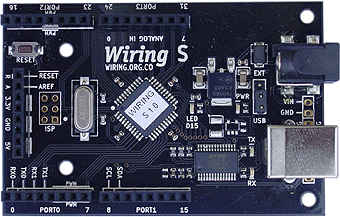
\includegraphics[scale=0.9]{artigo/refs/Rogue_BB_WRS}
	\end{center}
	%\legend{Fonte: Site da 3GPP}
\end{figure}
\section{Software Wiring}

% Verificar na própria tese do Barragàn os Tópicos 4 e 5. Já dá para adiantar que não será assunto suficiente, então será necessário dar uma pequena pesquisada. Não precisa ser longo o conteúdo
\section{A biblioteca Wiring no Arduíno}
\subsection{Principais Funções}
\chapter{Wiring e o AVR}

\section{Atmel AVR}

O AVR é um microcontrolador RISC desenvolvido pela Atmel e posteriormente comprado pela Microchip Tecnology. Possui uma pequena memória flash para armazenamento do programas e 32 registradores internos. Este tipo de chip é muito utilizado em hardwares de prototipagem, como o Arduíno.

Conforme \citeonline{borges2006desenvolvimento} "Com o objetivo de maximizar o desempenho e o paralelismo, o AVR segue arquitetura Harvard, em que os barramentos associados às memórias de dados e do programa são distintos. Além disso, utiliza-se a técnica do \emph{pipeline}, em que, enquanto uma instrução começa a ser executada, uma outra já é buscada na memória de programa para que a mesma possa ser executada no próximo ciclo de relógio"

Um microcontrolador possui internamente todas as caracteristicas de um computador possuindo processador, memória e periféricos de entrada e saída. Este tipo de circuito é conhecido como \emph{System-on-chip}. Esta característica o faz ser amplamente utilizado em hardwares de prototipagem pois possui características suficientes para a execução de programas e acionamento de pinos, por exemplo.

A versão mais popular do Arduíno, o Arduíno Uno, possui um microcontrolador ATmega328 (\autoref{atmega})

\begin{figure}[htb]
	\begin{center}
	    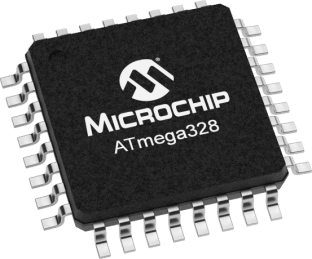
\includegraphics[scale=0.5]{artigo/refs/medium-ATmega328-TQFP-32.png}
	\end{center}
	\caption{\label{atmega}chip ATmega328}
	%\legend{Fonte: Site da 3GPP}
\end{figure}

Algumas das características do ATmega328 são listadas na tabela abaixo

\section{Programando para AVR}

No diretório de instalação do Arduíno há uma biblioteca denominada avr/io.h, esta biblioteca possui todas as diretivas para outras bibliotecas com base no microcontrolador utilizado. Nestas bibliotecas há definições de registradores de entrada e saída, pinos, constantes e diversos outros componentes, conforme trecho abaixo.

\subsection{Bibliotecas AVR}

Aqui um pequno trecho da biblioteca io.h em que, de acordo com o chip AVR utilizado, uma nova biblioteca é incluída.
\newline
\newline
\begin{lstlisting}
//biblioteca io.h
//(...)
#ifndef _AVR_IO_H_
#define _AVR_IO_H_

#include <avr/sfr_defs.h>

#if defined (__AVR_AT94K__)
#  include <avr/ioat94k.h>
//(...)
#elif defined (__AVR_ATmega328P__)
#  include <avr/iom328p.h>
#elif (defined __AVR_ATmega328__)
#include <avr/iom328.h>
//(...)

\end{lstlisting}
%INSERIR IMAGEM DO ATMEGA328, INSERIR TAMBÉM UM TRECHO OU OUTRO E FINALIZAR

Aqui um pequno trecho da biblioteca io.h em que, de acordo com o chip AVR utilizado, uma nova biblioteca é incluída.

\begin{lstlisting}
//biblioteca iom328p.h
//(...)
#ifndef _AVR_IOM328P_H_
#define _AVR_IOM328P_H_ 1

/* Registers and associated bit numbers */

#define PINB _SFR_IO8(0x03)
#define PINB0 0
//(...)
#define DDRB _SFR_IO8(0x04)
#define DDB0 0
#define DDB1 1
//(...)
#define PORTB _SFR_IO8(0x05)
#define PORTB0 0
#define PORTB1 1
//(...)
\end{lstlisting}

\section{Conclusão}



% ---
% Finaliza a parte no bookmark do PDF, para que se inicie o bookmark na raiz
% ---
\bookmarksetup{startatroot}% 
% ---

% ---
% Conclusão
% ---
\section*{Considerações finais}
%\addcontentsline{toc}{section}{Considerações finais}


Lorem ipsum dolor sit amet, consectetur adipiscing elit. Donec diam elit, pellentesque sit amet nunc at, eleifend elementum eros. Praesent pulvinar nibh turpis, eget faucibus lectus efficitur vel. Vivamus ut nisi risus. Class aptent taciti sociosqu ad litora torquent per conubia nostra, per inceptos himenaeos. Proin sed quam vitae risus vulputate auctor eget ut odio. Praesent eleifend porttitor purus, in ullamcorper neque placerat quis. Praesent fringilla enim lectus, vitae varius nunc cursus vitae. Praesent vitae ex vitae massa aliquet fringilla. Interdum et malesuada fames ac ante ipsum primis in faucibus. Nulla vehicula mi risus, eu sollicitudin dui bibendum non. Nam nec orci nec enim dapibus ullamcorper nec sed sapien.

Sed tincidunt, nunc vulputate lobortis commodo, sem massa auctor quam, et egestas erat dui in dui. Aenean efficitur, urna vitae condimentum placerat, dui dolor lobortis dui, nec molestie velit purus sed lorem. Quisque eu nunc tellus. Integer in risus accumsan, vehicula arcu quis, interdum velit. Aenean molestie congue dolor, at suscipit odio iaculis quis. Vestibulum posuere, leo vel aliquet pellentesque, risus metus rhoncus metus, at lobortis diam ipsum vel neque. Vivamus augue arcu, facilisis eu facilisis fermentum, eleifend non urna. Integer faucibus, odio eget dictum rhoncus, nisi augue volutpat libero, vitae cursus justo ex et metus. Ut eleifend lectus ut quam rhoncus blandit. Nunc maximus elit velit, varius facilisis ligula rutrum quis. Integer nec interdum purus. Duis finibus urna a elementum fringilla. Quisque eget porta mi, nec fringilla tellus. Quisque lacinia leo at diam tincidunt ornare. Suspendisse potenti. Nulla facilisi. Mauris. 

%\begin{citacao}[english]
 % "When you start monitoring the environment,
  %something happens: You start to understand the world around you in a %new way." \cite{Gertz2012}
%\end{citacao}





% ----------------------------------------------------------
% ELEMENTOS PÓS-TEXTUAIS
% ----------------------------------------------------------

% ]  				% FIM DE ARTIGO EM DUAS COLUNAS
% ---

% ----------------------------------------------------------
% Referências bibliográficas
% ----------------------------------------------------------
\bibliography{refs/refs.bib}

% ----------------------------------------------------------
% Glossário
% ----------------------------------------------------------
%
% Há diversas soluções prontas para glossário em LaTeX. 
% Consulte o manual do abnTeX2 para obter sugestões.
%
%\glossary

% ----------------------------------------------------------
% Apêndices
% ----------------------------------------------------------

% ---
% Inicia os apêndices
% ---
% ---

% ----------------------------------------------------------
% Anexos
% ----------------------------------------------------------

% ---
% Inicia os anexos
% ---
%\anexos
%\nocite{Wickham2018,Ross1996,Leek2016,Leek2015,Peng2015b}
\end{document}
